\chapter{Introduction}
\label{ch:introduction}
\pagenumbering{arabic}

This chapter introduces the motivation, problem setting, and research context of this work. It begins by outlining the limitations of current deep learning models in handling corrupted and clinically realistic time-series data. The chapter then presents an overview of related work in robustness benchmarking, calibration improvement techniques, and data augmentation for time series. Finally, it summarizes the core contributions of this work.

\section{Problem Statement}

The global burden of neurological disorders has intensified interest in automated techniques for analyzing brain activity. Among these disorders, epilepsy affects more than 50 million people worldwide~\cite{whoEpilepsy}. According to a 2017 population-based review~\cite{thurman2011standards}, the mean lifetime prevalence of epilepsy was estimated to be 7.6 per 1,000 people, making it one of the most common serious neurological conditions. Seizures, marked by sudden bursts of abnormal electrical brain activity, often require precise detection and localization for diagnosis and treatment. Electroencephalography (EEG) remains the most widely used clinical tool for this purpose, offering non-invasive insight into temporal brain dynamics through scalp-mounted electrodes~\cite{niedermeyer2005}.

In recent years, deep neural networks have achieved considerable success in EEG signal classification and seizure detection tasks~\cite{schirrmeister2017deep, roy2019chrononet}. However, their deployment in clinical settings faces two critical limitations. First, neural networks are highly sensitive to distributional shifts, such as noise corruptions, missing sensors, or patient movement artifacts, that deviate from the training distribution~\cite{ovadia2019can, hendrycks2019benchmarking}. Such perturbations are commonplace in clinical EEG and can severely degrade predictive accuracy. Second, modern networks often produce overconfident predictions, failing to reflect the true likelihood of correctness~\cite{guo2017calibration}. This miscalibration is particularly concerning in high-stakes domains like healthcare, where confidence estimates may directly influence clinical decisions.

While various techniques have been developed to improve robustness and calibration, the majority of these have been evaluated on benchmark image datasets (e.g., CIFAR-10-C, ImageNet-C~\cite{hendrycks2019benchmarking}) under synthetic perturbations. In contrast, EEG-specific benchmarks for evaluating model reliability under corruption remain underdeveloped. For example, the widely adopted Temple University Seizure Corpus (TUSZ)~\cite{obeid2016temple} lacks standardized corruption protocols for testing robustness under realistic EEG noise and signal degradation.

To address these limitations, this work proposes a novel benchmark that introduces controlled corruptions, including Gaussian noise, spectral augmentation, signal dropout, and channel dropout, designed to reflect imperfections commonly encountered in clinical EEG data. This benchmark facilitates rigorous and reproducible evaluation of robustness methods on time-series data, a domain in which such practices remain rare.

Several techniques that have demonstrated success in improving robustness in vision tasks include Mixup~\cite{thulasidasan2019mixup}, Manifold Mixup~\cite{manifoldmixup}, Multi-Input Multi-Output (MIMO)\cite{MIMO}, and Test-Time Adaptation (TTA)\cite{tta}. However, their effectiveness under realistic EEG corruption scenarios has not been systematically assessed. Furthermore, while individual methods have been studied in isolation, their combinatorial effects on robustness and calibration are not well understood. This work investigates not only individual method performance but also how their combinations aim to identify configurations that either enhance or compromise predictive accuracy and calibration under challenging EEG conditions.
\begin{figure}[htb]
	\centering
        \def\svgwidth{300pt}
 	\import{gfx/}{contributions.pdf_tex} 	  	 	
	\caption[Overview of the challenges and contributions of this work]{Overview of the problem, challenges, and contributions of this work.}
	\label{fig:overview}
\end{figure}

%***********Motivation and Context***********************
\section{Previous Work}
Deep learning has significantly advanced various fields, particularly in computer vision and natural language processing, achieving remarkable performance on benchmark datasets such as ImageNet \cite{deng2009imagenet}, CIFAR-10, and CIFAR-100 \cite{krizhevsky2009learning}. Despite successes under controlled conditions, neural networks often exhibit limited robustness when exposed to real-world corruptions or subtle distributional shifts. These vulnerabilities pose risks, particularly in safety-critical applications such as medical diagnostics, underscoring the need for systematic evaluation of model robustness and calibration \cite{hendrycks2019benchmarking}.

\subsection{Benchmarking Robustness and Calibration}
Robustness benchmarking systematically evaluates neural network performance under structured corruptions, simulating realistic variations and degradations in data quality. A key example in computer vision is the ImageNet-C benchmark proposed by Hendrycks and Dietterich \cite{hendrycks2019benchmarking}, comprising controlled corruptions including noise (Gaussian, impulse), blur (motion, defocus), weather distortions (snow, fog), and digital artifacts (JPEG compression, pixelation), each generated across multiple severity levels (see Figure~\ref{fig:imagenetC}). Extensions such as CIFAR-C and CIFAR-P further facilitate comparative assessments, inspiring advancements in training methods and network architectures \cite{hendrycks2019benchmarking}.

\begin{figure}[htb]
	\centering
 	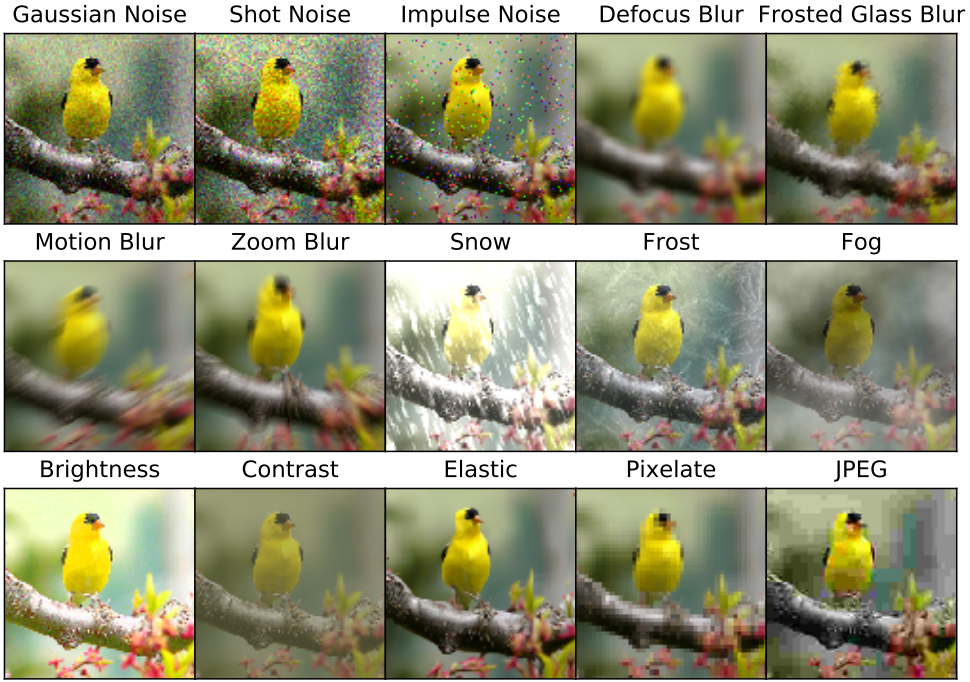
\includegraphics[width=0.9\textwidth]{gfx/fig1.png}  	  	 
	\caption[IMAGENET-C dataset consists of 15 types of corruptions]{Algorithmically generated corruptions categorized into digital, weather, blur, and noise distortions, each with varying severity levels~\cite{hendrycks2019benchmarking}.}
	\label{fig:imagenetC}
\end{figure}

Despite these advances in image-based benchmarking, equivalent structured robustness benchmarks for time-series data, particularly EEG signals, remain underdeveloped. EEG data's distinct temporal and spectral structures limit the applicability of image-based benchmarks, complicating the evaluation of model robustness in clinical EEG diagnostics like seizure detection, where noise, electrode dropouts, and artifacts pose significant challenges to diagnostic accuracy and reliability \cite{iwana2021empirical, lawhern2018eegnet}.

Thus, the establishment of dedicated EEG robustness benchmarks is essential for ensuring reliable and safe deployment of clinical EEG-based diagnostic systems.

\subsection{Methods to Improve Robustness and Calibration}
To address these robustness challenges, various general approaches have emerged within the machine learning community, aimed at enhancing model generalization and calibration under distributional shifts.

Regularization techniques are foundational, reducing overfitting by limiting model complexity and training convergence. Approaches such as weight decay, dropout, and early stopping effectively prevent neural networks from overfitting training data \cite{srivastava2014dropout, krogh1992simple}. Adversarial training, another critical regularization approach, introduces adversarially perturbed samples during training, significantly improving model resistance to adversarial inputs and data corruptions \cite{madry2017towards}.

Ensemble methods aggregate multiple model predictions, reducing variance and enhancing robustness. Approaches like bagging, boosting, and stacking combine diverse predictions, leading to improved calibration and stability by averaging individual model biases and errors \cite{lakshminarayanan2017simple}.

Bayesian neural networks quantify predictive uncertainty explicitly, utilizing probabilistic methods such as Monte Carlo dropout and variational inference. These methods provide calibrated predictions and reliable uncertainty estimates, essential for informed decision-making in critical applications \cite{gal2016dropout, blundell2015weight}.

Self-supervised learning methods further enhance robustness by learning generalizable feature representations without explicit supervision. Techniques such as contrastive learning and autoencoder-based methods effectively improve robustness to distributional shifts, particularly valuable when labeled data is scarce or noisy \cite{chen2020simple, grill2020bootstrap}.

Additionally, post-hoc calibration approaches like temperature scaling, isotonic regression, and Platt scaling adjust predicted probabilities, significantly enhancing confidence estimate reliability in high-stakes scenarios \cite{guo2017calibration}.

Despite broad coverage in general machine learning literature, these techniques remain insufficiently explored specifically for clinical EEG-based time-series analysis, marking a clear research gap that requires further exploration.

\subsection{Data Augmentation in Time Series}
Data augmentation has been instrumental in improving robustness and generalization in computer vision through techniques like flipping, rotation, scaling, cropping, and color jittering \cite{shorten2019survey}. However, directly applying such augmentations to time-series data is challenging due to inherent temporal dependencies and physiological constraints.

Time-series-specific augmentations have been proposed, including temporal jittering, scaling, permutation, and window slicing, preserving meaningful temporal structures \cite{iwana2021empirical}. Additionally, frequency-domain augmentations, notably SpecAugment, mask contiguous frequency and time segments, effectively enhancing robustness to noise and distortions \cite{spectral_aug}.

Advanced augmentation methods involve synthetic data generation using generative adversarial networks (GANs), generating plausible synthetic time-series data to mitigate class imbalance \cite{esteban2017realvalued}. Moreover, adapted mixup techniques generate virtual samples through interpolation, promoting smoother decision boundaries and improved generalization in time-series applications \cite{um2017data}.

In EEG classification, however, data augmentation is applied inconsistently, limiting reproducibility and systematic evaluation. While techniques like random cropping and channel shuffling have shown potential, standardized and comprehensive evaluations under corrupted conditions remain scarce.

Consequently, developing standardized evaluation frameworks for EEG-specific augmentation methods is crucial, ensuring robust, reproducible, and clinically relevant EEG classification systems.


%***********Contributions**********
\section{This Work's Contributions}
This work presents several key contributions toward improving the robustness and calibration of deep neural networks for EEG time series classification:

\begin{itemize}
    \item \textbf{EEG Corruption Benchmark:} To address the lack of standardized evaluation protocols for robustness in EEG classification, this work introduces a novel benchmark comprising controlled corruptions such as Gaussian noise, spectral augmentation, channel dropout, and signal dropout, explicitly designed to simulate real-world EEG imperfections encountered in clinical settings.

    \item \textbf{Systematic Robustness Evaluation:} Using the proposed benchmark, this work conducts a comprehensive assessment of state-of-the-art robustness enhancement techniques, including Mixup, Manifold Mixup, Multi-Input Multi-Output (MIMO), and Test-Time Adaptation (TTA).

    \item \textbf{Calibration Analysis and Metrics:} This work rigorously evaluates both predictive performance and confidence reliability using metrics such as accuracy, F1 score, and Expected Calibration Error (ECE), providing a nuanced understanding of model behavior under distributional shifts.

    \item \textbf{Method Compatibility and Combination Effects:} In addition to isolated evaluations, this work explores how robustness techniques interact when combined. Notably, performance degradation in specific combinations (e.g., MIMO with Manifold Mixup) highlights the importance of compatibility-aware design.
\end{itemize}
\begin{figure}[h!]
	\centering
        \def\svgwidth{400pt}
        \fontsize{7pt}{7pt}
 	\import{gfx/}{approach.pdf_tex} 	  	 	
	\caption[Overview of the structure of this work]{Overview of the structure of this work.}
	\label{fig:approach}
\end{figure}

\subsection*{This Work’s Structure}
This work is organized as follows. Chapter~\ref{ch:background} introduces the foundational concepts relevant to this work, including EEG, neural networks, calibration, and robustness. Chapter~\ref{ch:methodology} presents the proposed methodology, detailing the dataset, preprocessing steps, robustness-enhancing model variants, and the corruption techniques used to simulate real-world EEG imperfections. Evaluation protocols and calibration metrics are also discussed. Chapter~\ref{ch:results} reports the experimental results, focusing on performance under distribution shifts, calibration behavior, and the effects of method combinations. Chapter~\ref{ch:discussion} provides a critical discussion of findings and limitations. Finally, Chapter~\ref{ch:closure} concludes this work and outlines potential directions for future research.

